\chapter{Mecánica Estadística}


\section{Fundamentos estadísticos de la Termodinámica}
\begin{itemize}
	\item La especificación de los valores de los parámetros $N$, $V$ y $E$
	define a un \textbf{macroestado}.
	
	\item Los \textbf{microestados} se identifican como las posibles 
	configuraciones de un sistema para dar lugar al mismo valor 
	de energía $E$ del sistema completo, $\Omega=\Omega(N,V,E).$
	
	\item \textbf{Postulado de la igualdad de probabilidad apriori:} el sistema
	tiene igualdad de probabilidad de estar en cualquiera de los posibles
	microestados.
	
	\item Al colocar dos sistemas termodinámicos en contacto se supone
	que estos llegarán al equilibrio cuando se el valor de la energía
	del sistema (\janote{del sistema?}) maximice el número 
	de microestados en los que se puede encontrar el sistema.
	El macroestado con la mayor cantidad de microestados 
	se dice que es el más probable.
	
	\item $S=k\ln \Omega$: entropía absoluta en términos del número
	total de microestados accesibles según el macroestado del sistema.
	
	\item De la fórmula que enunció Planck sobre la entropía (ya había
	sido formulada por Boltzmann, pero fue Planck quien la escribió en la
	forma moderna) se desprende que la entropía se hace cero cuando 
	el sistema puede encontrarse en una sola configuración.
	
	\item \textbf{El gas ideal clásico}: dado que asumimos que las 
	partículas no interactúan entre sí dentro del gas, entonces
	\begin{align}
	\Omega (N,E,V)\propto V^N,
	\end{align}
	y esto nos lleva a que 
	\begin{align}
	\pdv{S}{V}&=\frac{P}{T}=k\qty(\pdv{\ln \Omega \qty(N,E,V)}{V})_{N,E}=
	k\frac{N}{V}  \\
	PV&=kNT = nRT \hspace{1.5cm} (R=kN_A),
	\end{align}
	así hemos llegado a la ecuación de estado del gas ideal desde 
	principios estadísticos.
	
	\item \textbf{Paradoja de Gibbs (entropía de mezcla):} Gibbs consideró
	una situación como la de la \Fref{fig:gibbs-paradox} en la que 2 gases
	iguales se mantienen a ambos lados de una pared diatérmana, luego
	la pared se quita y se permite que ambos gases se mezclen. En este 
	caso particular tenemos un proceso reversible porque podemos 
	volver a colocar la pared y tendríamos la misma situación inicial. 
	Sin embargo, con métodos estadísticos se concluye que la diferencia
	de entropía entre los estados inicial y final del sistema total es distinto
	de cero, lo que contradice lo bien conocido de la termodinámica 
	de que en un proceso reversible adiabático el cambio en la 
	entropía es igual a cero. La propuesta de Gibbs para resolver
	esta paradoja fue cambiar la expresión de la entropía $S$ de 
	un gas ideal de 
	\begin{align}
	S(N,V,E)=Nk\ln\qty[\frac{V}{h^3}\qty(\frac{4\pi mE}{3N})^{3/2}]
	+\frac{3}{2}Nk
	\end{align}
	a
	\begin{align}
	S(N,V,E)=Nk\ln\qty[\frac{V}{Nh^3}\qty(\frac{4\pi mE}{N})^{3/2}]
	+\frac{5}{2}Nk,
	\end{align}
	habiendo así agregado de manera \textit{ad hoc} los términos
	$-k\ln N!$ $(\approx Nk\ln N-Nk)$.
	\begin{figure}
	    \centering
	    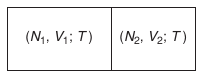
\includegraphics[width=5cm]{images/mixing-2gases.png}
	    \caption{Mezcla de dos gases ideales.}
	    \label{fig:gibbs-paradox}
	  \end{figure}
	  
	\item La consecuencia física del arreglo de Gibbs es que se está 
	reduciendo el número de microestados accesibles por el sistema 
	en un factor $N!$. La justificación de esto es que estamos lidiando
  con partículas idénticas que son indistinguibles, por consiguiente
  no tiene sentido etiquetar individualmente a cada una de las
  partículas. Todo lo que podemos contar es la distribución 
  sobre los estados de energía.
\end{itemize}

\section{Elementos de la teoría de los ensambles}
\begin{itemize}
	\item Un microestado de un sistema clásico, en un tiempo $t$, está
	definido por las posiciones y momenta de todas las partículas
	que constituyen al sistema.
	\item Las coordenadas $(q_i,p_i)$ representan un punto en 
	un espacio de $6N$ dimensiones conocido como el espacio de fases.
	\item Función de densidad $\rho(q,p;t)$: para describir mejor 
	los ensambles de microestados en los que se puede encontrar
	un sistema. Esta función es tal que el número de puntos 
	representativos dentro del elemento de volumen $d^{3N}qd^{3N}p$
	alrededor del punto $(q,p)$ del espacio de fases está dado por 
	el proudcto $\rho(q,p;t)d^{3N}qd^{3N}p$.
	\item El promedio del ensamble $\expval{f}$ de una cantidad
	física $f(q,p)$ está dado por 
	\begin{align}
	\expval{f}=
	\frac{\int f(q,p)\rho(q,p;t)d^{3N}qd^{3N}p}{\int \rho(q,p;t)d^{3N}qd^{3N}p}
	\end{align}
	
	\item \textbf{Teorema de Liouville:} Consideremos una región de
	volumen arbitrario $\omega$, cuya superficie la vamos a denotar
	por $\sigma$, como se ve en la \Fref{fig:liouville}. 
	Entonces, la tasa a la que el número de puntos 
	representativos en este elemento de volumen aumenta con 
	el tiempo es
	\begin{align}
	\pdv{t}\int_{\omega} \rho d\omega.
	\end{align}
	Por otro lado, el flujo hacia afuera de $\omega$ está dado por 
	\begin{align}
	\int _{\sigma}\rho \vb{v}\cdot \vb{\hat{n}}d\sigma.
	\end{align}
	Por el teorema de la divergencia (que no tengo fresco en el momento
	que estoy escribiendo esto \janote{OJO}) tenemos 
	\begin{align}
	\int _\omega \div{\rho \vb{v}}d\omega.
	\end{align}
	En vista que no hay fuentes ni sumideros
	\begin{align}
	\pdv{t}\int_{\omega} \rho d\omega=-\int _\omega \div{\rho \vb{v}}d\omega,
	\end{align}
	por lo que 
	\begin{align}
	\int _{\omega}\qty(\pdv{\rho}{t}+\div{\rho\vb{v}})d\omega=0.
	\end{align}
	Por lo cual, inmediatamente se tiene 
	\begin{align}
	\pdv{\rho}{t}+\div{\rho\vb{v}}=0,
	\end{align}
	y esta ecuación es conocida como la ecuación de continuidad. 
	Trabajando más esta ecuación 
	\begin{align}
	\pdv{\rho}{t}+\sum_{i=1}^{3N}
	\qty(\pdv{\rho}{q_i}\dot{q}_i+\pdv{\rho}{p_i}\dot{p}_i)+
	\rho \sum_{i=1}^{3N}
	\qty(\pdv{\dot{q}_i}{q_i} + \pdv{\dot{p}_i}{p_i})=0.
	\end{align}
	\h{Recordatorio eqs. de Hamilton:} 
	\begin{align}
	\dot{q}_i&=\pdv{H(q_i,p_i)}{p_i}\\
	\dot{p}_i&=-\pdv{H(q_i,p_i)}{q_i}.
	\end{align}
	Usando la ecuaciones de Hamilton notamos que 
	el tercer término en la ecuación de continuidad se hace cero,
	por consiguiente llegamos al resultado 
	conocido como el \h{teorema de Liouville}:
	\begin{align}
	\pdv{\rho}{t}+\{\rho,H\}=0,
	\end{align}
	donde $\{\rho,H\}$ es el bracket de Poisson. La consecuencia 
	física de este teorema es que las trayectorias en el espacio de 
	fases se mueven de la misma manera que un fluido 
	incompresible.
	\begin{figure}
	  \centering
	  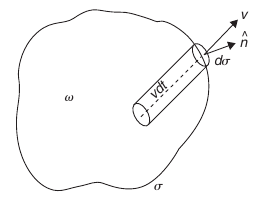
\includegraphics[width=5cm]{images/phase-space.png}
	  \caption{Elemento de volumen en el espacio de fases.}
	  \label{fig:liouville}
	\end{figure}
	
	\item \textbf{Ensamble canónico:} $E=$ cte.
	
	\item \textbf{El ensamble microcanónico:}
	El macroestado del ensamble microcanónico de un sistema está 
	definido por el número de moléculas $N$, el volumen $V$ y la 
	energía $E$. El ensamble microcanónico es una colección de
	sistemas para los cuales la función de densidad $\rho$ está 
	dada por 
	\begin{align}
	\rho(q,p)=\text{cte.}\hspace{1cm}
	\text{si} \hspace{2mm}
	\qty(E-\frac{1}{2}\Delta)\leq
	H(q,p)\leq
	\qty(E+\frac{1}{2}\Delta).
	\end{align}
	
	\item El resultado fundamental es llegar a la \textbf{energía 
	libre de Helmholtz!!!!} (ver sec. 3.3 Pathria)
	
	\item El formalismo del ensamble microcanónico y canónico son equivalentes.
	
	\item \textbf{Teorema de equipartición:} (revisar notas en Drive para la 
	deducción matemática) cada término armónico en el Hamiltoniano 
	transformado de un sistema contribuye $1/2kT$ a la energía 
	interna del sistema. Dicho de otro modo, cada grado de libertad 
	aporta la misma cantidad al valor esperado de la energía del sistema 
	total. \textbf{No obstante}, el teorema de equipartición es válido 
	para valores de temperatura muy altos, osea cuando los 
	grados de libertad relevantes del sistema pueden 
	ser excitados libremente.
	
	\item \textbf{Teorema del virial:} (revisar notas en Driva para la 
	deducción) 
	\begin{align}
	-\expval{\sum_iq_i\dot{p_i}}=3NkT,
	\end{align}
	donde
	\begin{align}
	\mathcal{V}=-3NkT,
	\end{align}
	es	llamado el 'virial' del sistema.
	Cuando se considera a un gas ideal esto se reduce a la relación 
	clásica:
	\begin{align}
	\mathcal{V}=-2K,
	\end{align}
	con $K$ la energía cinética del sistema.	
\end{itemize}

\subsection{Osciladores armónicos}
Asumiendo osciladores armónicos en una dimensión el hamiltoniano
$H$ del sistema es 
\begin{align}
H(q_i,p_i)=\sum_i\frac{1}{2}m\omega^2q_i^2+\frac{1}{2m}p_i^2.
\end{align}
Al calcular la función de partición $\mathcal{Z}$ de un oscilador armónico
\begin{align}
\mathcal{Z}&=\int _{-\infty}^{\infty}\int _{-\infty}^{\infty}
\exp\qty[-\beta\qty(\frac{1}{2}m\omega^2q^2+\frac{1}{2m}p^2)]
\frac{dqdp}{h}\nonumber\\
&=\frac{1}{h}\qty(\frac{2\pi}{\beta m\omega^2})^{1/2}
\qty(\frac{2\pi m}{\beta})^{1/2}=
\frac{1}{\beta\hbar\omega}=\frac{kT}{\hbar\omega}.
\end{align}
De manera que entonces la función de partición del sistema 
completo es 
\begin{align}
\mathcal{Z}=\qty(\frac{kT}{\hbar\omega})^N.
\end{align}
La energía libre de Helmholtz está dada por 
\begin{align}
A&=-kT\ln \mathcal{Z}\nonumber\\
&=-NkT\ln\qty(\frac{kT}{\hbar\omega}).
\end{align}
De manera que las otras variables termodinámicas son
\begin{align}
S&=-\qty(\pdv{A}{T})_{N,V}\nonumber\\
&=Nk\qty[\ln\qty(\frac{kT}{\hbar\omega})+1]
\end{align}
y 
\begin{align}
U&=\pdv{\ln\mathcal{Z}}{\beta}\nonumber\\
&=NkT.
\end{align}

\section{Gran función de partición}
\subsection{Potencial químico}
Si se agrega una partícula a un sistema, entonces su energía interna
cambiará una cantidad que definimos como el \textbf{potencial químico}
$\mu$. Así que cuando este es el caso la primera y segunda ley de la
termodinámica se deben de modificar, agregando un término extra:
\begin{align}
\d U=T\d S-P\d V+\mu \d N,
\label{eq:dU-with-mu}
\end{align}
donde $N$ es el número de partículas del sistema. Esto inmediatamente 
implica que podemos escribir 
\begin{align}
\mu=\qty(\pdv{U}{N})_{S,V}.
\end{align}
Recordemos que la energía libre de Helmholtz se define como 
$A=U-TS$ y la energía libre de Gibbs como $G=U-PV-TS$, por consiguiente
\begin{align}
\d F&=-P\d V -S\d T+\mu \d N\\
\d G&=V\d P-S\d T+\mu\d N,
\end{align}
con lo cual se tiene 
\begin{align}
\mu &=\qty(\pdv{F}{N})_{V,T}\\
\mu &=\qty(\pdv{G}{N})_{P,T},
\end{align}
de manera que esta última expresión para $\mu$ en términos de la energía
libre de Gibbs se volverá particularmente útil dado que mantener las variables 
$P$ y $T$ constantes es algo viable en el experimento.

Podemos considerar que la función de entropía es $S=S(U,V,N)$,
de tal forma que 
\begin{align}
\d S=\qty(\pdv{S}{U})_{N,V}\d U+
\qty(\pdv{S}{V})_{N,U}\d V+
\qty(\pdv{S}{N})_{U,V}\d N.
\end{align}
Si dividimos la ecuación \eqref{eq:dU-with-mu} dentro de $T$ y 
despejamos para $\d S$ se tiene
\begin{align}
\d S=\frac{\d U}{T}+\frac{P\d V}{T}-\frac{\mu\d N}{T},
\end{align}
y al compararlo con la ecuación anterior podemos concluir que 
\begin{align}
\qty(\pdv{S}{U})_{N,V}&=\frac{1}{T} &
\qty(\pdv{S}{V})_{N,U} &=\frac{P}{T} &
\qty(\pdv{S}{N})_{U,V} &=-\frac{\mu}{T}.	
\end{align}